


\tikzset{every picture/.style={line width=0.75pt}} %set default line width to 0.75pt        

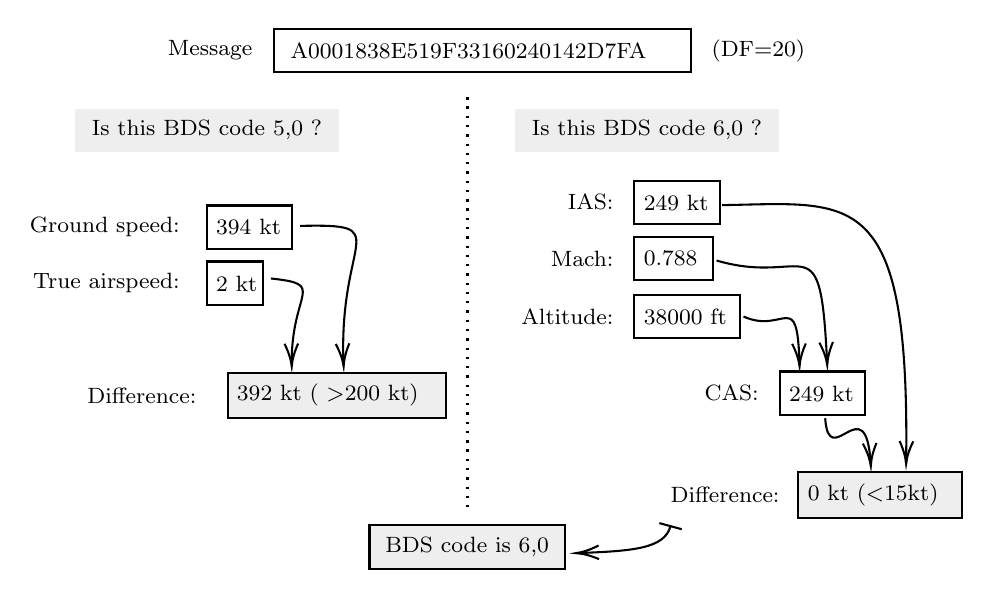
\begin{tikzpicture}[x=0.75pt,y=0.75pt,yscale=-1,xscale=1]
%uncomment if require: \path (0,348); %set diagram left start at 0, and has height of 348

%Curve Lines [id:da6430793918846669] 
\draw    (355.67,127) .. controls (399.45,139.94) and (405.61,106.34) .. (408.95,176.27) ;
\draw [shift={(409,177.33)}, rotate = 267.32] [color={rgb, 255:red, 0; green, 0; blue, 0 }  ][line width=0.75]    (10.93,-3.29) .. controls (6.95,-1.4) and (3.31,-0.3) .. (0,0) .. controls (3.31,0.3) and (6.95,1.4) .. (10.93,3.29)   ;
%Curve Lines [id:da32235700877254647] 
\draw    (368.67,154) .. controls (388.37,162.87) and (394.48,139.71) .. (395.62,176.29) ;
\draw [shift={(395.67,178)}, rotate = 268.53] [color={rgb, 255:red, 0; green, 0; blue, 0 }  ][line width=0.75]    (10.93,-3.29) .. controls (6.95,-1.4) and (3.31,-0.3) .. (0,0) .. controls (3.31,0.3) and (6.95,1.4) .. (10.93,3.29)   ;
%Curve Lines [id:da8301342497366322] 
\draw    (408,203) .. controls (409.97,229.6) and (427.46,187.3) .. (429.9,224.26) ;
\draw [shift={(430,226)}, rotate = 267.14] [color={rgb, 255:red, 0; green, 0; blue, 0 }  ][line width=0.75]    (10.93,-3.29) .. controls (6.95,-1.4) and (3.31,-0.3) .. (0,0) .. controls (3.31,0.3) and (6.95,1.4) .. (10.93,3.29)   ;
%Curve Lines [id:da14303571391445913] 
\draw    (358.33,100.33) .. controls (421.33,99.33) and (449,90) .. (447,225) ;
\draw [shift={(447,225)}, rotate = 270.85] [color={rgb, 255:red, 0; green, 0; blue, 0 }  ][line width=0.75]    (10.93,-3.29) .. controls (6.95,-1.4) and (3.31,-0.3) .. (0,0) .. controls (3.31,0.3) and (6.95,1.4) .. (10.93,3.29)   ;
%Curve Lines [id:da7746471843860618] 
\draw    (141,135.67) .. controls (168.25,138.62) and (150.87,141.25) .. (150.98,176.37) ;
\draw [shift={(151,178)}, rotate = 268.96] [color={rgb, 255:red, 0; green, 0; blue, 0 }  ][line width=0.75]    (10.93,-3.29) .. controls (6.95,-1.4) and (3.31,-0.3) .. (0,0) .. controls (3.31,0.3) and (6.95,1.4) .. (10.93,3.29)   ;
%Curve Lines [id:da5542954001907279] 
\draw    (155,110.33) .. controls (201.53,109.34) and (173.57,114.89) .. (175.92,176.13) ;
\draw [shift={(176,178)}, rotate = 267.27] [color={rgb, 255:red, 0; green, 0; blue, 0 }  ][line width=0.75]    (10.93,-3.29) .. controls (6.95,-1.4) and (3.31,-0.3) .. (0,0) .. controls (3.31,0.3) and (6.95,1.4) .. (10.93,3.29)   ;
%Straight Lines [id:da3827685237283216] 
\draw  [dash pattern={on 0.84pt off 2.51pt}]  (235.67,48.33) -- (235.67,249) ;
%Curve Lines [id:da8658759276112653] 
\draw    (333.5,255) .. controls (330.56,265.78) and (315.62,266.96) .. (289.61,267.94) ;
\draw [shift={(288,268)}, rotate = 357.88] [color={rgb, 255:red, 0; green, 0; blue, 0 }  ][line width=0.75]    (10.93,-3.29) .. controls (6.95,-1.4) and (3.31,-0.3) .. (0,0) .. controls (3.31,0.3) and (6.95,1.4) .. (10.93,3.29)   ;
\draw [shift={(333.5,255)}, rotate = 285.26] [color={rgb, 255:red, 0; green, 0; blue, 0 }  ][line width=0.75]    (0,5.59) -- (0,-5.59)   ;

% Text Node
\draw    (142.26,15.33) -- (343.26,15.33) -- (343.26,36.33) -- (142.26,36.33) -- cycle  ;
\draw (145.26,25.83) node [anchor=west] [inner sep=0.75pt]  [font=\footnotesize] [align=left] {\begin{minipage}[lt]{134.18644pt}\setlength\topsep{0pt}
\begin{center}
A0001838E519F33160240142D7FA
\end{center}

\end{minipage}};
% Text Node
\draw (133.51,25.83) node [anchor=east] [inner sep=0.75pt]  [font=\footnotesize] [align=left] {Message};
% Text Node
\draw    (110.12,100.5) -- (151.12,100.5) -- (151.12,121.5) -- (110.12,121.5) -- cycle  ;
\draw (113.12,111) node [anchor=west] [inner sep=0.75pt]  [font=\footnotesize] [align=left] {394 kt};
% Text Node
\draw (98.52,111) node [anchor=east] [inner sep=0.75pt]  [font=\footnotesize] [align=left] {Ground speed:};
% Text Node
\draw    (110.12,127.5) -- (137.12,127.5) -- (137.12,148.5) -- (110.12,148.5) -- cycle  ;
\draw (113.12,138) node [anchor=west] [inner sep=0.75pt]  [font=\footnotesize] [align=left] {2 kt};
% Text Node
\draw (98.52,138) node [anchor=east] [inner sep=0.75pt]  [font=\footnotesize] [align=left] {True airspeed:};
% Text Node
\draw    (316.12,88.5) -- (357.12,88.5) -- (357.12,109.5) -- (316.12,109.5) -- cycle  ;
\draw (319.12,99) node [anchor=west] [inner sep=0.75pt]  [font=\footnotesize] [align=left] {249 kt};
% Text Node
\draw (307.52,99) node [anchor=east] [inner sep=0.75pt]  [font=\footnotesize] [align=left] {IAS:};
% Text Node
\draw    (316.12,115.5) -- (354.12,115.5) -- (354.12,136.5) -- (316.12,136.5) -- cycle  ;
\draw (319.12,126) node [anchor=west] [inner sep=0.75pt]  [font=\footnotesize] [align=left] {0.788};
% Text Node
\draw (307.52,126) node [anchor=east] [inner sep=0.75pt]  [font=\footnotesize] [align=left] {Mach:};
% Text Node
\draw    (386.12,180.5) -- (427.12,180.5) -- (427.12,201.5) -- (386.12,201.5) -- cycle  ;
\draw (389.12,191) node [anchor=west] [inner sep=0.75pt]  [font=\footnotesize] [align=left] {249 kt};
% Text Node
\draw (377.52,191) node [anchor=east] [inner sep=0.75pt]  [font=\footnotesize] [align=left] {CAS:};
% Text Node
\draw    (316.12,143.5) -- (367.12,143.5) -- (367.12,164.5) -- (316.12,164.5) -- cycle  ;
\draw (319.12,154) node [anchor=west] [inner sep=0.75pt]  [font=\footnotesize] [align=left] {38000 ft};
% Text Node
\draw (307.52,154) node [anchor=east] [inner sep=0.75pt]  [font=\footnotesize] [align=left] {Altitude:};
% Text Node
\draw  [fill={rgb, 255:red, 238; green, 238; blue, 238 }  ,fill opacity=1 ][line width=0.75]   (120.12,181) -- (225.12,181) -- (225.12,203) -- (120.12,203) -- cycle  ;
\draw (123.12,192) node [anchor=west] [inner sep=0.75pt]  [font=\footnotesize] [align=left] {392 kt ( $\displaystyle  >$200 kt)};
% Text Node
\draw (106.52,192) node [anchor=east] [inner sep=0.75pt]  [font=\footnotesize] [align=left] {Difference:};
% Text Node
\draw  [fill={rgb, 255:red, 238; green, 238; blue, 238 }  ,fill opacity=1 ][line width=0.75]   (395.12,229) -- (474.12,229) -- (474.12,251) -- (395.12,251) -- cycle  ;
\draw (398.12,240) node [anchor=west] [inner sep=0.75pt]  [font=\footnotesize] [align=left] {0 kt ($\displaystyle < $15kt)};
% Text Node
\draw (387.52,240) node [anchor=east] [inner sep=0.75pt]  [font=\footnotesize] [align=left] {Difference:};
% Text Node
\draw  [draw opacity=0][fill={rgb, 255:red, 238; green, 238; blue, 238 }  ,fill opacity=1 ]  (46.65,53.83) -- (173.65,53.83) -- (173.65,74.83) -- (46.65,74.83) -- cycle  ;
\draw (110.15,64.33) node  [font=\footnotesize] [align=left] {Is this BDS code 5,0 ?};
% Text Node
\draw  [draw opacity=0][fill={rgb, 255:red, 238; green, 238; blue, 238 }  ,fill opacity=1 ]  (258.65,53.83) -- (385.65,53.83) -- (385.65,74.83) -- (258.65,74.83) -- cycle  ;
\draw (322.15,64.33) node  [font=\footnotesize] [align=left] {Is this BDS code 6,0 ?};
% Text Node
\draw  [color={rgb, 255:red, 0; green, 0; blue, 0 }  ,draw opacity=1 ][fill={rgb, 255:red, 238; green, 238; blue, 238 }  ,fill opacity=1 ]  (188.48,254.5) -- (282.48,254.5) -- (282.48,275.5) -- (188.48,275.5) -- cycle  ;
\draw (235.48,265) node  [font=\footnotesize] [align=left] {BDS code is 6,0};
% Text Node
\draw (351.8,25.83) node [anchor=west] [inner sep=0.75pt]  [font=\footnotesize] [align=left] {(DF=20)};


\end{tikzpicture}
